%!TEX root = slides.tex
%!TEX program = xelatex
% (für das LaTeXtools Sublime plugin)

\documentclass{beamer}

\usepackage{csquotes}
\usepackage{braket}

%Blablabla front matter....

\title{Quantum Key Distribution}
\subtitle{Foundational Aspects of Quantum Mechanics}
\date{01-02-2017}
\author[Hirscher, Snijders]{Simon Hirscher \& Max Snijders}

%\setbeameroption{show notes}
%\setbeamertemplate{note page}[plain]

\usepackage[LastSlideNotCounted,ProgressBar,NoPageCounter]{beamer-template-mk-i/beamerthememxmki}
\hypersetup{pdfpagemode=FullScreen}

% Use this for the handout!

% \usepackage{pgfpages}
% \pgfpagesuselayout{4 on 1}[a4paper]

% Diagonal arrows
\usepackage{mathtools}
\newcommand{\myarrow}[1][-45]{%
  \mathrel{%
    \text{$
     \begin{tikzpicture}[baseline = -0.5ex]
       \node[inner sep=0pt,outer sep=0pt,rotate = #1] (a) at (0,0)  {$\leftrightarrow{}$};
    \end{tikzpicture}
    $}%
  }%
}%

% Color mix
\definecolor{sharedsecretcolor}{RGB}{191,178,64}
\definecolor{bobrandomseed}{RGB}{0,237,255}
\definecolor{bobmix}{RGB}{128,237,128}

% Quotes are awesome! (Sometimes)

\newcommand*{\openquote}{\tikz[remember picture,overlay,xshift=-15pt,yshift=-10pt]
	\node (OQ) {\fontsize{60}{60}\selectfont``};\kern0pt}
\newcommand*{\closequote}{\tikz[remember picture,overlay,xshift=15pt,yshift=10pt]
	\node (CQ) {\fontsize{60}{60}\selectfont''};}
% select a colour for the shading
\definecolor{shadecolor}{named}{white}
% wrap everything in its own environment
\newenvironment{shadequote}%
{\begin{quote}\openquote}
		{\hfill\closequote\end{quote}}


% And now for the real deal...
\begin{document}
	% commented out so it doesn't appear in the table of contents
	%\section{Introduction} % Simon

	\begin{frame}
		% Empty slide for talk start
	\end{frame}

	\begin{frame}
		\begin{center}
		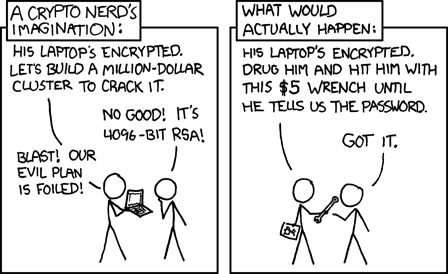
\includegraphics[width=0.8\textwidth]{images/xkcd-security.png}
		\end{center}
	\end{frame}

	\begin{frame}
		\titlepage
	\end{frame}

	% Structure of the talk
	\begin{frame}{Contents} % Simon
		\tableofcontents
	\end{frame}

	\section{Introduction to Encryption}
	\begin{frame}{The setting}
		Alice and Bob
	\end{frame}

	\begin{frame}{What is Encryption?} % Simon
		\begin{equation}
			\operatorname{ENC}: \underset{\cong\;\mathbb{N}}{\{\text{plaintexts}\}}
						\overset{\text{bijective}}{\longrightarrow}
						\underset{\cong\;\mathbb{N}}{\{\text{ciphertexts
						}\}}
						% \subset
						% \underset{\cong\;\mathbb{N}}{\{\text{cipher-like
						% texts}\}}
						\nonumber
		\end{equation}
		\begin{itemize}
			\item The function should be easily reversible for the
			recipient but impossible to reverse for a 3rd party

 			\item \textbf{Symmetric encryption:} $\operatorname{ENC}$
 			and $\operatorname{ENC}^{-1}$ are generated from one secret
 			number, referred to as \textbf{the shared secret} or
 			\textbf{secret key}.

 			\item \textbf{Asymmetric encryption:} $\operatorname{ENC}$
 			is generated from a \textbf{public key}, known to everyone
 			and specific to the recipient, $\operatorname{ENC}^{-1}$
 			generated from a \textbf{private key}, known only to the
 			recipient.

		\end{itemize}
	\end{frame}

	\begin{frame}{Shifting Caesar Cipher} % Max
		\begin{columns}
			\begin{column}{0.7\textwidth}
				\begin{figure}
					\begin{tikzpicture}[scale=1, every node/.style={scale=1}]
					    \node[anchor=center,inner sep=0] at (-0.08,-0.00) {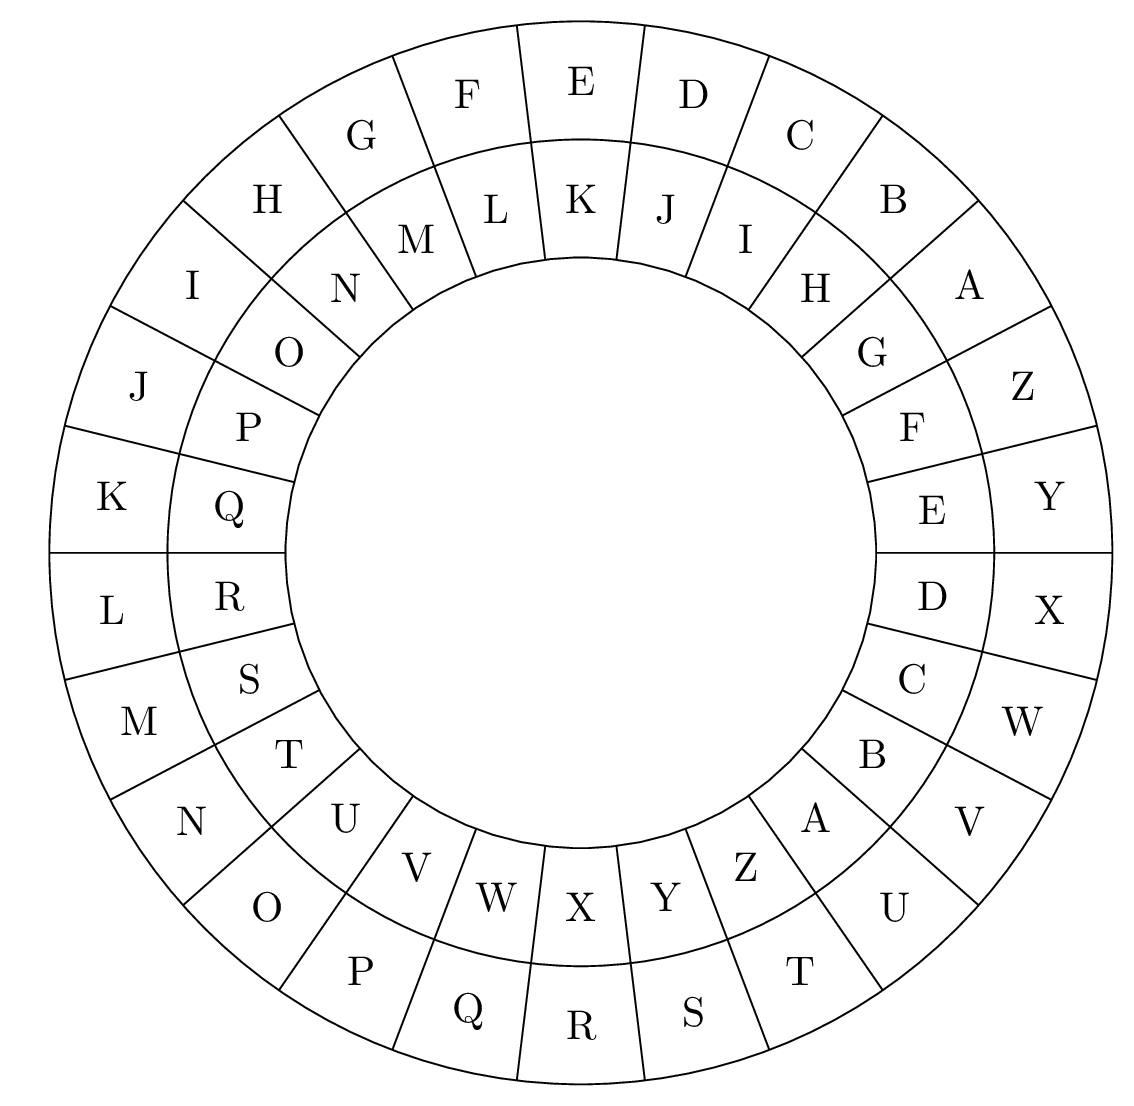
\includegraphics[width=0.85\textwidth]{images/shifting-caesar-cipher}};

					    \draw[fill = Bordeaux, thick] (0,0) circle(0.1);

					    \onslide<3->{\draw[Bordeaux, thick,->, opacity=0.5] (0:0) -- (48.5:2.37);}
						\onslide<2->{\draw[Bordeaux, ultra thick,->,opacity=1.0] (0:0) -- (48.5:1.69);}

						\onslide<5->{\draw[Bordeaux, thick,->, opacity=0.5] (0:0) -- (6.9:2.37);}
						\onslide<4->{\draw[Bordeaux, ultra thick,->,opacity=1.0] (0:0) -- (6.9:1.69);}

						\onslide<7->{\draw[Bordeaux, thick,->, opacity=0.5] (0:0) -- (103.8:2.37);}
						\onslide<6->{\draw[Bordeaux, ultra thick,->,opacity=1.0] (0:0) -- (103.8:1.69);}

						\onslide<9->{\draw[Bordeaux, thick,->, opacity=0.5] (0:0) -- (145.4:2.37);}
						\onslide<8->{\draw[Bordeaux, ultra thick,->,opacity=1.0] (0:0) -- (145.4:1.69);}

						\onslide<11->{\draw[Bordeaux, ultra thick, ->] (-48.5:3.2) arc (-48.5:34.6:3.2);}

						\onslide<11->{\node[rotate=-100, Bordeaux] at (-10:3.5) {\textbf{Key}};}
					\end{tikzpicture}
				\end{figure}
			\end{column}
			\begin{column}{0.4\textwidth}
				\begin{itemize}
					\onslide<10->\item \enquote{HELLO} $\rightarrow$ \enquote{BYFFI}
					\onslide<12->\item 26 options
					\onslide<13->\item Vulnerable to \textbf{brute-force} attack.
					\onslide<13->\item Vulnerable to \textbf{frequency analysis}.
					\onslide<13->\item Vulnerable to \textbf{known plaintext} attacks.
				\end{itemize}
			\end{column}
		\end{columns}
	\end{frame}

	\begin{frame}{Permutation Cipher} % Max
		\begin{columns}
			\begin{column}{0.5\textwidth}
				\begin{figure}
					\begin{table}
						\begin{tabular}{ c | c }
							Plaintext & Ciphertext \\
							\hline
							\onslide<2->{A & G \\}
							\onslide<3->{B & X \\}
							\onslide<4->{C & C \\}
							\onslide<5->{D & J \\}
							\onslide<6->{\vdots & \vdots}
						\end{tabular}
					\end{table}
				\end{figure}
			\end{column}
			\begin{column}{0.5\textwidth}
				\begin{itemize}
					\onslide<7->\item \enquote{ABBACD} $\rightarrow$ \enquote{GXXGCJ}
					\onslide<8->\item $26 \cdot 25 \cdot 24 \cdot \hdots \cdot 1 = 26! \approx 10^{26}$ options
					\onslide<9->\item Vulnerable to \textbf{frequency analysis}.
					\onslide<9->\item Vulnerable to \textbf{known plaintext} attacks.
				\end{itemize}
			\end{column}
		\end{columns}
	\end{frame}

	\begin{frame}{XOR} % Simon

	\end{frame}

	\begin{frame}{One-Time Pad} % Simon
		One-time pad = random key of size $n$ ($n=$ length of message),
		only used once.

		\begin{table}
			\begin{tabular}{l | c c c c c c c c }
				Bit \#     & 1 & 2 & 3 & 4 & \onslide<2->{5} & \onslide<3->{6} & \onslide<4->{$\hdots$} & \onslide<5->{$n$} \\
				\hline
				Plaintext  & 1 & 0 & 1 & 1 & \onslide<2->{1} & \onslide<3->{0} & \onslide<4->{$\hdots$} & \onslide<5->{1} \\
				%\hline
				Key        & 1 & 1 & 0 & 1 & \onslide<2->{0} & \onslide<3->{1} & \onslide<4->{$\hdots$} & \onslide<5->{1} \\
				%\hline
				Ciphertext & 0 & 1 & 1 & 0 & \onslide<2->{1} & \onslide<3->{1} & \onslide<4->{$\hdots$} & \onslide<5->{0} \\
			\end{tabular}
		\end{table}

		\textbf{Unbreakable} \onslide<6>{since:}

		\only<7>{\vspace{1em}\begin{center}
\includegraphics[width=0.2\textwidth]{images/obama_not_bad.jpg}\end{center}}

		\onslide<6>{No correlation between encrypted bits at positions i and j (or
		between subsequent encrypted messages). \linebreak $\implies$
		Every possible plaintext can be obtained from the ciphertext by
		choosing the right key. \linebreak $\implies$ No way to find out
		whether key / plaintext is correct.}

		\vspace{3em}

	\end{frame}

	% Key distribution section
	\section{Key Distribution}
	\begin{frame}{The problem with exchanging the key} % Simon
		% "So we've found the perfect encryption. What's the problem?"

		How do we agree on the key in the first place? How can we do that securely?\linebreak

		\onslide<2->{Two ways:}

		\begin{enumerate}
			\onslide<2->{
			\item Meet in person every time we want to exchange a
			message. \only<3>{
			% Look of disapproval ಠ_ಠ
			% Download the "Kedage" font here: http://brahmi.sourceforge.net/
			% \vspace{1em}
			% \begin{center}
			% \fontsize{50pt}{12pt}
			\textbf{{\fontspec{Kedage} ಠ}\_{\fontspec{Kedage} ಠ}}
			% \end{center}
			}
			}

			\onslide<4->{
			\item Meet in person once, exchange a whole stack of paper
			with a lot of keys for a lot of future messages.
			}
		\end{enumerate}

		\onslide<5->{
		Okay, we don't actually have to meet in person…
		}

	\end{frame}

%	\begin{frame}{Diffie-Hellman Key Exchange (DHE)} % Max
%		\begin{columns}
%			\begin{column}{\textwidth}
%				\begin{figure}
%					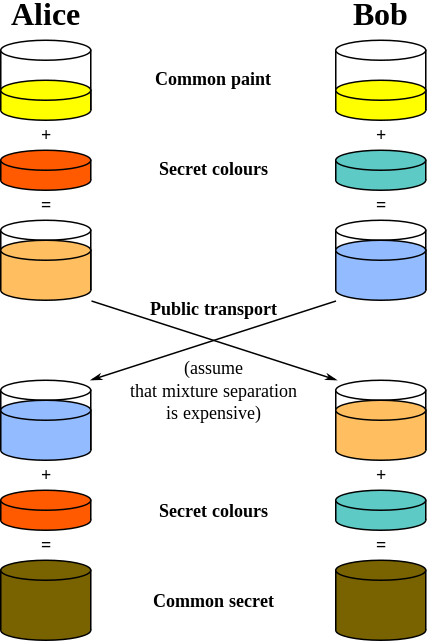
\includegraphics[width=0.4\textwidth]{images/diffie-hellman}
%				\end{figure}
%			\end{column}
%		\end{columns}
%	\end{frame}


	\begin{frame}{Diffie-Hellman Key Exchange (DHE)} % Max
		\begin{columns}
			\begin{column}{\textwidth}
				\vspace{-20pt}
				\begin{figure}
					\scalebox{0.42}{\hspace{-40pt}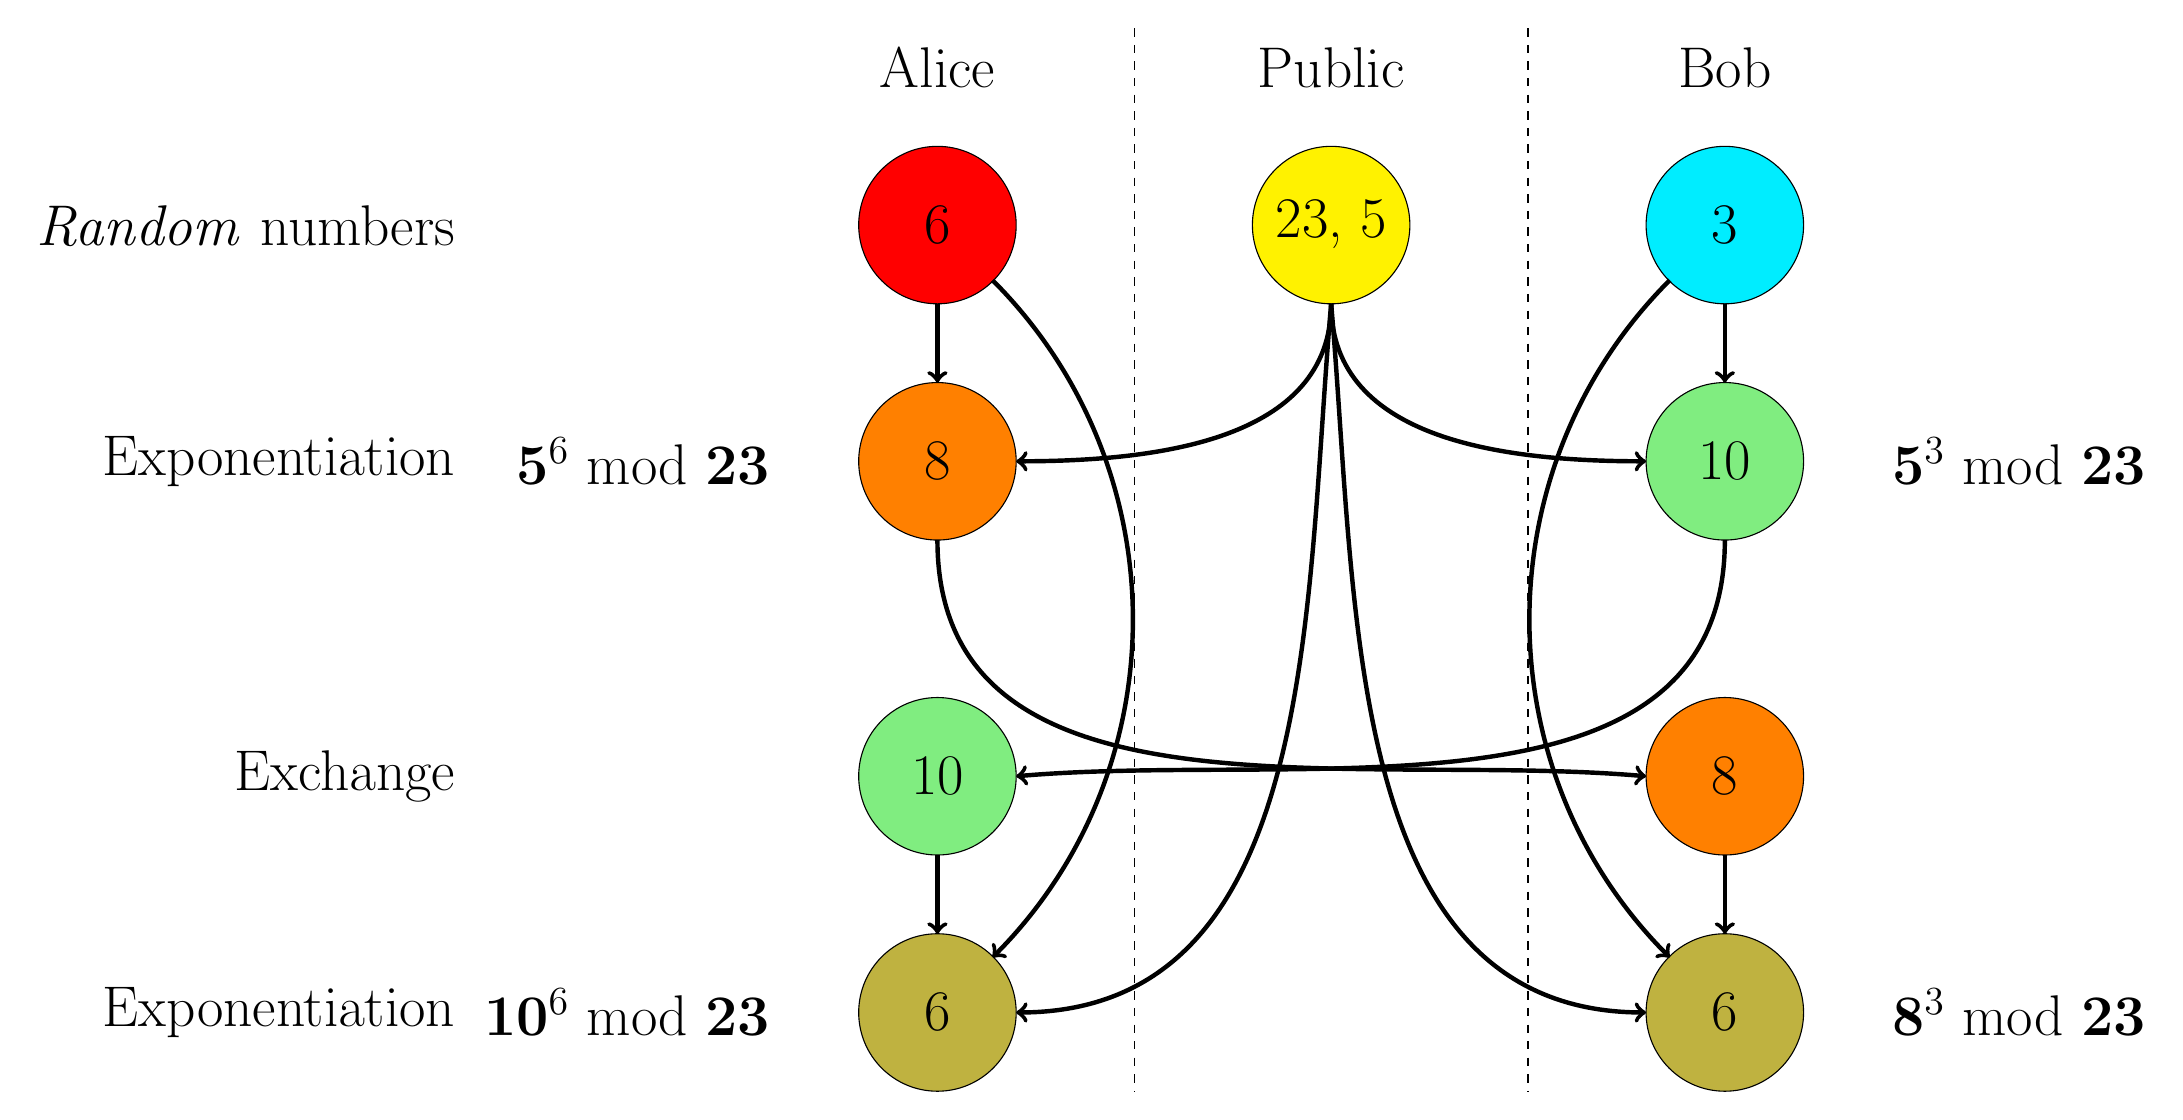
\begin{tikzpicture}
					
						\node at (0,2) {\huge Public};
						\node at (-5,2) {\huge Alice};
						\node at (5,2) {\huge Bob};
						
						\draw[fill = yellow] (0,0) circle(1);
						
						\node at (0,0) {\huge 23, 5};

						\node[anchor=east] at (-11,0) {\huge \textit{Random} numbers};

						\onslide<2->{
							\draw[fill = red] (-5,0) circle(1);
							\draw[fill = bobrandomseed]  ( 5,0) circle(1);
							\node at (-5,0) {\huge 6};		
							\node at (5,0) {\huge 3};
						}
						
						\onslide<3->{
							\draw[fill = orange] (-5,-3) circle(1);
							\draw[fill = bobmix] (5,-3) circle(1);
							\node[anchor=east] at (-11,-3) {\huge Exponentiation};
							\node[anchor=east] at (-7,-3) {\huge \textbf{5}\textsuperscript{6} mod \textbf{23}};
							\node at(-5,-3) {\huge 8};
							\node at(5,-3) {\huge 10};
							\node[anchor=west] at (7,-3) {\huge \textbf{5}\textsuperscript{3} mod \textbf{23}};
							\draw[->, ultra thick] (-5,-1) -- (-5,-2);
							\draw[->, ultra thick] (0,-1) to[out=-90,in=0] (-4,-3);
							\draw[->, ultra thick] (5,-1) -- (5,-2);
							\draw[->, ultra thick] (0,-1) to[out=-90,in=180] (4,-3);
						}
						
						\onslide<4->{
							\draw[fill = bobmix] (-5,-7) circle(1);
							\draw[fill = orange] (5,-7) circle(1);
							\node[anchor=east] at (-11,-7) {\huge Exchange};
							\node at(-5,-7) {\huge 10};
							\node at(5,-7) {\huge 8};
							\draw[->, ultra thick] (-5,-4) to[out=-90,in=175] (4,-7);
							\draw[->, ultra thick] (5,-4) to[out=-90,in=5] (-4,-7);
						}
						
						\onslide<6->{
							\draw[fill = sharedsecretcolor] (-5,-10) circle(1);
							\draw[fill = sharedsecretcolor] (5,-10) circle(1);
							\node[anchor=east] at (-11,-10) {\huge  Exponentiation};
							\node at(-5,-10) {\huge 6};
							\node at(5,-10) {\huge 6};
							\draw[->, ultra thick] (-5,-8) -- (-5,-9);
							\draw[->, ultra thick] (5,-8) -- (5,-9);
							\draw[->,ultra thick] (-4.3,-0.7) to[out=-45,in=45] (-4.3,-9.3);
							\draw[->,ultra thick] (4.3,-0.7) to[out=-135,in=135] (4.3,-9.3);
							\draw[->,ultra thick] (0,-1) to[out=-85,in=-180] (4,-10);
							\draw[->,ultra thick] (0,-1) to[out=-95,in=0] (-4,-10);
							
							\node[anchor=east] at (-7,-10) {\huge \textbf{10}\textsuperscript{6} mod \textbf{23}};
							\node[anchor=west] at (7,-10) {\huge \textbf{8}\textsuperscript{3} mod \textbf{23}};

						}

						\draw[dashed] (-2.5,2.5) -- (-2.5,-11);
						\draw[dashed] ( 2.5,2.5) -- ( 2.5,-11);
						
						
					\end{tikzpicture}}
				\end{figure}
			\end{column}
		\end{columns}
	\end{frame}
	
	\begin{frame}{Diffie-Hellman Details} % Max
		\begin{itemize}
			\onslide<2->{
				\item Choice of the two publicly known numbers not random: exponentiation and then taking the modulus should have maximum range and spread:
					\begin{align*}
						5^n \; \text{mod} \; 23 = \; &\mathbf{1}, \mathbf{5}, 2, 10, 4, 20, 8, 17, 16, 11, 9, 22, \\&18, 21, 13, 19, 3, 15, 6, 7, 12, 14, \mathbf{1}, \mathbf{5}, \hdots
					\end{align*}
			}
			
			\onslide<3->{
				\item Exponentiation is easy to compute, hard to invert. (Last week's talk)
			}
			
			\onslide<4->{
				\item Impractical for one-time pad use
			}
		\end{itemize}
	\end{frame}


	% \begin{frame}{Public/Private Key} % Simon

	% \end{frame}

	% Methods of Quantum Key Exchange
	\section{Quantum Key Distribution}

	\begin{frame}{Quantum Key Distribution}
		QKD makes use of fundamental principles of quantum mechanics:

		\begin{enumerate}
			\item<2-> Measurement changes system {\tiny (unless in
			eigenstate of observable)}

			\begin{itemize}
				\item<3-> existence of such measurement guaranteed by
				existence of complementary observables
			\end{itemize}

			\item<4-> No-cloning theorem $\rightarrow$ will prevent Eve
			from eavesdropping / copying the key material
		\end{enumerate}
	\end{frame}

	\begin{frame}{No-cloning theorem}
		\begin{itemize}
			\item Consider two Hilbert spaces $H_A \cong H_B$,
			$\operatorname{dim}H_A \geq 2$.

			\item Want to find unitary operator (time evolution) $U$
			such that $\forall \ket{\psi} \in H_A, \ket{b} \in H_B: U(\ket{\psi} \otimes \ket{b}) \overset{!}{=} \ket{\psi} \otimes \ket{\psi}$ (up to a phase)
			
			\item But then take another $\ket{\phi} \in H_A$:
				\begin{align*}
					\braket{\psi|\phi} = \braket{\psi|\phi}\braket{b|b} &= \big(\bra{\psi} \otimes \bra{b}\big) \big(\ket{\phi} \otimes \ket{b}\big) \\
					&= \big(\bra{\psi} \otimes \bra{b}\big) U^\dagger U \big(\ket{\phi} \otimes \ket{b}\big) \\
					&= \big(\bra{\psi} \otimes \bra{\psi}\big) \big(\ket{\phi} \otimes \ket{\phi}\big)
					= \braket{\psi|\phi}^2
				\end{align*}

				$\implies \braket{\psi|\phi} = 1$, i.e. identical, or $\braket{\psi|\phi} = 0$ \\
				$\implies$ Can never work with different, non-orthogonal states

			% \item But then for $\ket{\psi} \coloneqq \frac{1}{\sqrt{2}}(\ket{\psi_1} + \ket{\psi_2})$:
			% 	\begin{align*}
			% 		U(\ket{\psi} \otimes \ket{b}) &\overset{\text{Def.}}{=} \ket{\psi} \otimes \ket{\psi} \overset{\text{expand}}{=} \text{4 terms} \\
			% 		U(\ket{\psi} \otimes \ket{b}) &\overset{\text{lin.}}{=} \frac{1}{\sqrt{2}}( U(\ket{\psi_1} \otimes \ket{b}) + U(\ket{\psi_2} \otimes \ket{b})) \\
			% 		&= \frac{1}{\sqrt{2}}( \ket{\psi_1} \otimes \ket{\psi_1} + \ket{\psi_2} \otimes \ket{\psi_2})
			% 		&= \text{2 terms} 
			% 	\end{align*}

		\end{itemize}
	\end{frame}


	\begin{frame}{BB-84 Protocol} % Max
		\begin{columns}
			\begin{column}{\textwidth}
				\begin{enumerate}
					\item For each bit in the message:
						\begin{enumerate}
							\item Alice picks a basis B randomly
							\item Alice transmits the bit V using this basis
							\item Bob measures the bit V using a randomly chosen basis B.
						\end{enumerate}
					\item Alice and Bob exchange a list of chosen bases.
					\item Where the chosen bases match Alice and Bob append the sent / measured bit to the shared key
				\end{enumerate}
			\end{column}
		\end{columns}
	\end{frame}
	
	\begin{frame}{BB-84 Example} % Max
		\begin{columns}
			\begin{column}{0.7\textwidth}
				\begin{table}
					\begin{tabular}{r | c | c | c | c  }
						Bit no. & 1 & 2 & 3 & 4 \\
						\hline
						Alice's random data & 0 & 1 & 1 & 0 \\
						Alice's random bases & 1 & 1 & 1 & 0 \\
						Bob's random bases & 0 & 1 & 0 & 0 \\
						\hline
						Alice's sent values & $\myarrow[45]$ & $\myarrow[-45]$ & $\myarrow[-45]$ & $\myarrow[0]$ \\
						Bob's measured values & ? & 1 & ? & 0 \\
						\hline
						Shared key & - & 1 & - & 0 
					\end{tabular}
				\end{table}
			\end{column}
			\vrule{}
			\begin{column}{0.3\textwidth}
				\begin{table}
					\begin{tabular}{c | c  c}
						 B \textbackslash \; V & 0 & 1 \\
						  \hline
						0 & $\myarrow[0]$ & $\myarrow[90]$ \\
						1 & $\myarrow[45]$ & $\myarrow[-45]$ \\
					\end{tabular}
	
				\end{table}

			\end{column}
		\end{columns}
	\end{frame}
	
	\begin{frame}{BB-84 Intercept-Resend Attack} % Max
		\begin{columns}
			\begin{column}{0.3\textwidth}
				\begin{table}
					\begin{tabular}{c | c | c}
						A's Basis & E's & B's \\
						\hline
						0 & 0 & 0 \\
						0 & 0 & 1 \\
						0 & 1 & 0 \\
						0 & 1 & 1 \\
						1 & 0 & 0 \\
						1 & 0 & 1 \\
						1 & 1 & 1
					\end{tabular}
				\end{table}
			\end{column}
			\begin{column}{0.7\textwidth}
				\begin{itemize}
					\onslide<2->{\item If all bases match Eve is not detectable}
					\onslide<3->{\item If Alice and Bob's bases don't match Eve is not detectable}
					\onslide<4->{\item If Alice and Bob's bases do match but Eve's is different then Bob will measure Alice's value 50\% of the time.}
				\end{itemize}
				\onslide<5->{$\implies$ Alice and Bob will match values when their bases match \textbf{75\%} of the time. \\}
				\onslide<6->{$\implies$ Alice and Bob will match values when their bases don't match \textbf{50\%} of the time.}
			\end{column}

	
		\end{columns}
	\end{frame}
	
	\begin{frame}{BB84 - Another Attack}
		\begin{itemize}
			\item \onslide<1->{Let's say Eve picks a different basis}
			\item \onslide<2->{Example on the board}
		\end{itemize}
	\end{frame}
	
	\begin{frame}{BB84 - Error correction}
		\begin{itemize}
			\item In practice: Transmissions errorneous
			\item Moreover, we saw: Eve can eavesdrop at the expense of
			introducing errors among bits where bases were matched at
			rate of 25\%
		\end{itemize}
		$\implies$ To detect Eve:
		\begin{itemize}
			\item Keep systematic error rate (noise level $N$) far below
			25\%
			\item Publicly compare small part of the key and compute
			error rate $E$
			\begin{itemize}
				\item $E > N \implies$ discard key
				\item $E \sim N \implies$ do error correction and proceed
			\end{itemize}
		\end{itemize}
	\end{frame}

	\begin{frame}{BB84 - Privacy amplification}
		Situation:
		\begin{itemize}
			\item Assume error rate was low and Alice and Bob now have
			same key
			\item Eve might still have partial knowledge of the key
		\end{itemize}

		\onslide<2->{
			Reduce her knowledge further through \textbf{privacy amplification}:
			\begin{itemize}
				\item<3-> Publicly announce positions $i, j$ of two bits $b_i, b_j$
				\item<4-> Replace bit $i$ with $\operatorname{XOR}(b_i, b_j)$,
				discard bit $j$.
			\end{itemize}
		}
		\onslide<5->{
			$\implies$ Eve's average knowledge of
			the key \textbf{decreases} at the expense of decreasing the
			key length. \onslide<6->{$\rightarrow$ blackboard}
		}
	\end{frame}


	\begin{frame}{BB-84 Properties} % Max
		\begin{itemize}
			\item Matching values percentage indicator of noise / eavesdroppers
			\item Only useful for setting up a secure channel, no authentication use
			\item On-the-fly one time pad generation
			\item In practice: over 300 km @ 12.7 kbits/second through optical fiber.
		\end{itemize}
	\end{frame}

	\begin{frame}{E-91} % Simon

	\end{frame}

	% Authentication Requirement
	\section{Authentication}

	\begin{frame}{Public/Private Key Authentication} % Simon

	\end{frame}

	% Hacks
	\section{Vulnerabilities}

	\begin{frame}{Vulnerabilities} % Max
		\begin{itemize}
			\item Basis choice leak							
			\item Authentication issues
			\item Pseudo-randomness of basis choice
		\end{itemize}
	\end{frame}

	% Closing
	\section{Closing}

	\begin{frame}
		\begin{center}
		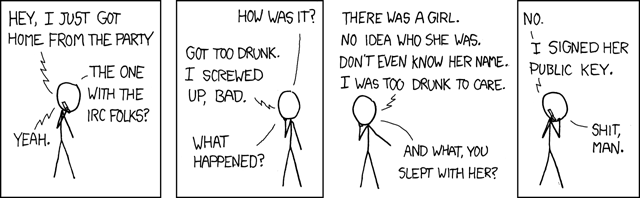
\includegraphics[width=\textwidth]{images/xkcd-responsible_behavior}
		\end{center}
	\end{frame}


	% A black slide to end the talk
	\setbeamercolor{background canvas}{bg=black}
	\begin{frame}[plain]\end{frame}

\end{document}